\section{Introduction}
\label{section:introduction}

The distributed ledger ecosystem continues to evolve,
 bringing about an increase in both the complexity of decentralized applications
 and the requirements for system throughput. 
The most robust solutions, which have proven their security through years of stable operation, 
 now face the challenge of evolving at a pace 
 that does not compromise the decentralization 
 inherent in the original protocol.
The Ethereum Network is the main example of these challenges,
 suffering from network congestion and high transaction fees. 
To mitigate these issues, Layer 2 solutions have been introduced.
These protocols extend the original protocol to enhance scalability 
 while inheriting the security of the Layer 1 network.

 The current strategy to address the scaling issues leans heavily on the
 concept of modularity through rollups and data availability and consensus layers.
While this approach has shown promise, existing solutions introduce significant drawbacks.
Rollups are segregated by design, 
 leading to fragmentation in terms of security, liquidity, and data consistency.
Furthermore, the need to redeploy applications from Ethereum to a Layer 2 solution
 exacerbates liquidity fragmentation. 
Additionally, rollups are not scalable in themselves 
 and require an additional rollup-on-top-of-rollup to achieve scalability. 

This document introduces zkSharding, 
 a Layer 2 architecture capable of scaling the Layer 1 network as needed 
 without causing fragmentation. 
This is made possible through several key components:
\begin{itemize}
    \item Parallel execution of transactions across different shards 
     by distinct sets of validators, 
     enabling a high throughput of up to 60,000 transactions per second; 
    \item Zero Knowledge state transition proofs that secure the system, 
     allowing validator sets to operate independently on shards 
     and verify other shards in a stateless manner; 
    \item An efficient consensus algorithm that facilitates cross-shard communication, 
     thus reducing transaction processing times. 
\end{itemize}

As illustrated in Figure \ref{figure:overview}, 
 the state of zkSharding is partitioned into the \mainshard and several execution shards. 
The \mainshard’s role is to synchronize and consolidate data 
 from the execution shards.
It uses Ethereum both as its Data Availability Layer and as a verifier for state transition proofs,
 similar to zkRollups operations.

Execution shards function as "workers", executing user transactions. 
These shards maintain unified liquidity and data through a cross-shard messaging protocol, 
 eliminating any fragmentation amongst them.
Each shard is supervised by a committee of validators. 
There is a periodic rotation of these validators across shards. 
In addition, updates to a shard’s state are verified 
 to the \mainshard using VM state transaction proofs

\begin{figure}
    \centering
	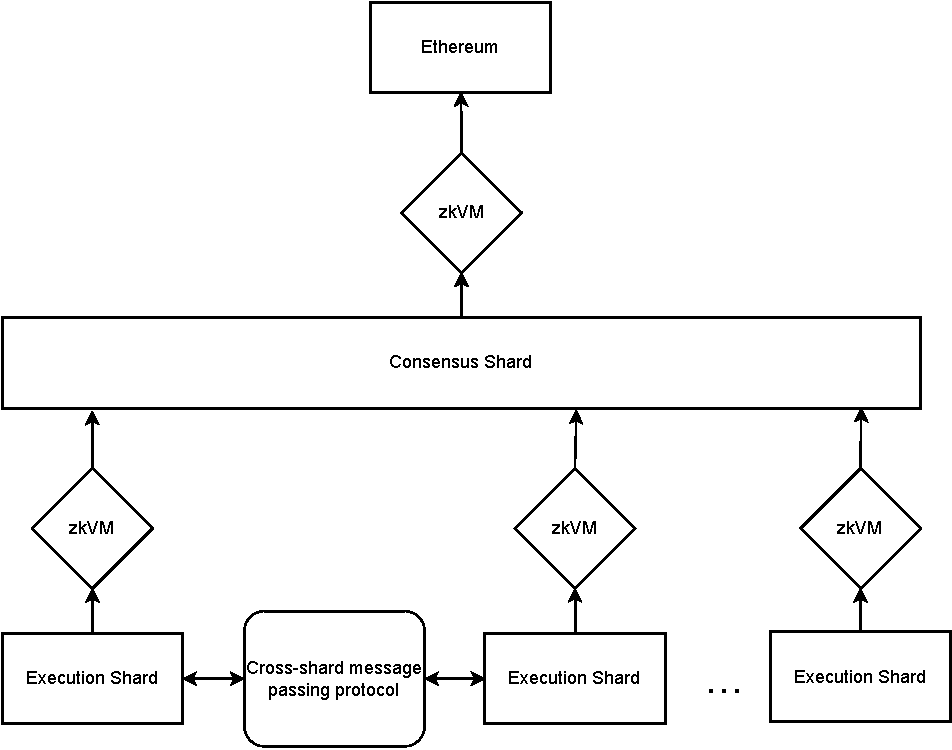
\includegraphics[scale=0.8]{figures/overview.drawio.pdf}
    \caption{zkSharding Architecture}
     \label{figure:overview}
\end{figure}

The zkSharding architecture serves as a foundation for \nil\ -- a zk-powered Layer 2 solution for scaling Ethereum. 

Section \ref{section:preliminaries} introduces fundamental definitions 
 and the models within which the protocol operates.
Section \ref{section:local-consensus} discusses how individual shards achieve consensus 
 and process transactions within Byzantine Fault Tolerant (BFT) settings.
Section \ref{section:sharding} explains the collaboration among shards 
 to ensure global security guarantees.
Section \ref{section:colocation} explores techniques aimed at 
 reducing transaction processing times in sharded configurations.
Section \ref{section:based-sequencer} describes the sequencing of transactions for zkSharding, 
 including how zkSharding's Data Availability transactions are ordered on Ethereum.
Section \ref{section:data-availability} delves into the Data Availability 
 mechanism utilized by zkSharding and provides an overview of Layer-1 finalization.
Section \ref{section:zk} examines the state transition proof mechanism 
 employed for dual purposes: Layer-2 state finalization and the inheritance of security from Layer-1.